% LaTeX template for the UNECE Worksession on Statistical Data Editing 2015, Budapest
% Last changed: 2015-04-10
% Author: Matthias Templ (using an earlier version by Steven Vale and Daniel Kilchmann)
% Revision and modification by Frederic Picard, Statistics Canada
% April 10 2015
% Revision and modification by Daniel Kilchmann, Swiss Federal Statistical Office
% December 7 2016, April 5 2018, October 8 2019, May 18 2022,

% DISCLAIMER: The UNECE document class style and the LaTeX-template
% are provided without any warranty at all and without any commitment
% to maintain or correct the code. In no event are UNECE or the
% author liable for any damages arising from the use of it.

% The uneceart document class style must be used for right numbering etc.
\documentclass[a4paper,11pt]{template/style/uneceart}

\usepackage{template/style/UNECE2023}
\usepackage{enumerate}
\usepackage{xcolor}

\definecolor{unece_color}{RGB}{84, 141, 212}

%%% ----------------------------------------------------------------------
%%% ---   please fill-in your personal data:   ---------------------------

%% the title of your contribution in capital letters:
\newcommand{\TITLE}{\textbf{Title} \\}

%% author:
\newcommand{\AUTHOR}{Author(s)}

%% your organisation
\newcommand{\ORGANISATION}{(Institution, Country or Organisation)}
\newcommand{\EMAIL}{e-mail}

%% abstract
\newcommand{\ABSTRACT}{Abstract text}


\begin{document}
%% Cover page with title and abstract
%%% by Matthias Templ, Vienna University of Technology, March 13, 2012. Updated Frederic Picard, Statistics Canada, March 09, 2015. Updated D. Kilchmann, SFSO, 7.12.2016, 5.4.2018., 8.10.2020, 6.4.2022
%%% Updated by Peter-Paul de Wolf for use in UNECE/Eruostat SDC meetings, 15.03.2023

\setcounter{page}{1}
\thispagestyle{empty} \vspace*{-2.0cm} %[width=0.65\textwidth]

\includegraphics[height=1.5cm]{template/UNECE_logo}\hspace*{8cm}
\includegraphics[height=1.5cm]{template/ModernStatsLogo}\\[\baselineskip]
%\hspace*{13cm} Working Paper \\
%\hspace*{13cm}ENGLISH ONLY\\\\
\textsc{UNITED NATIONS ECONOMIC COMMISSION FOR EUROPE} \vspace*{2mm}\\
\textsc{CONFERENCE OF EUROPEAN STATISTICIANS}\vspace*{2mm}\\
\textbf{Expert meeting on Statistical Data Confidentiality}\vspace*{2mm}\\
26--28 September 2023, Wiesbaden              %% check whether it is the right place and date
\vspace*{-1mm}
{\color{unece_color} \par\noindent\rule{\textwidth}{1.25pt}}\\[1cm]
%\TOPIC
%\begin{center}
{\LARGE \TITLE}\vspace*{-2mm}\\ %17pt
%\TYPE
\AUTHOR\ \\%11pt
% \ORGANISATION\vspace{2mm}\\ %11pt
\EMAIL\vspace*{1cm}\\ %11pt
%\end{center}
\noindent
{\large\textbf{\textit{Abstract}}}\\ %12pt
\ABSTRACT
\newpage



%% Real content of the paper
% Introduction
\section{Introduction}  %% The extra hspace is only to align the numbering more or less

Here is one paragraph of the introduction.

Here is a second paragraph of the introduction.

% First section
\section{Primary heading}
\subsection{Secondary heading} \label{sc:A}
Here is a paragraph.


\subsection{Secondary heading} \label{sc:B}
In this paragraph, we cite this book,
\cite{Hundepoolea2012}, but Figure~\ref{plot:1} is not taken from that book. Another paper contains some formulas \citep[see][]{Zhou2010Smoothing}. Also,
\begin{enumerate}
\item Xxxxxxxx
\begin{itemize}
\item Xxxxx
\begin{enumerate}
\item Yyyyy
\end{enumerate}
\item Xxxxx
\end{itemize}
\item Xxxxxxxxxxxxxxxxxx
\item Xxxxxxxxxxxxxxxxxx
\end{enumerate}


\section{Primary heading}

\subsection{Secondary heading}

This paragraph is a pretext to include a table:

\begin{tabular}{l*{6}{c}r}
Team              & P & W & D & L & F  & A & Pts \\
\hline
Manchester United & 6 & 4 & 0 & 2 & 10 & 5 & 12  \\
Celtic            & 6 & 3 & 0 & 3 &  8 & 9 &  9  \\
Benfica           & 6 & 2 & 1 & 3 &  7 & 8 &  7  \\
FC Copenhagen     & 6 & 2 & 1 & 2 &  5 & 8 &  7  \\
\end{tabular}


Another paragraph with high-flying content, maybe refering to
Section~\ref{sc:A}. We forgot to mention that
Figure~\ref{plot:1}  has been produced with \R .

\begin{figure}[ht]
\begin{center}
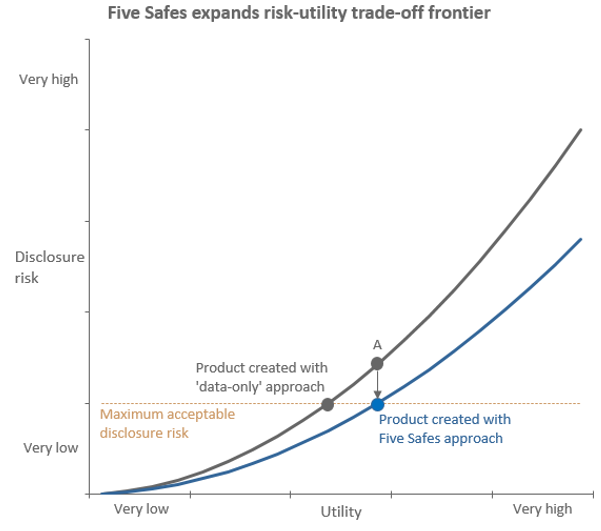
\includegraphics[width=0.65\textwidth]{template/figures/RU-5safes.png}
\caption{\label{plot:1}The Five Safes expands the R-U trade-off frontier. For each level of utility, we can achieve lower disclosure risk.\\
See \small{\url{https://www.abs.gov.au/statistics/research/confidentiality-abs-microdata}}}
\end{center}
\end{figure}

\bibliographystyle{chicago}
\bibliography{UNECE_template_2023SDC}

\end{document}
